\chapter{Literature Overview}
\label{cha:lit_overview}

%\section{Theoretical Framework}

As the thesis is in nature a research and experimental project the theory will mostly be used as a reference in how internals of the Linux system work and how to approach analyzing them.

\section{Key studies}

\begin{enumerate}
    \item {Linux manual pages}

    These pages can be accessed via any Linux distribution, but thanks to efforts by Michael Kerrisk they are also available online.
    These pieces of documentation are key in understanding specific Linux system concepts and how the system components work and interact with each other.

    \item {Open source libraries and their documentation}

    Due to the open source licensing of the Rust and Linux system, most of the libraries in the ecosystem are not only open source but also very well documented.
    This proved extremely helpful, as it allowed for ease of use and swift integration of dependencies into the project.
    Additionally, with the code of the said libraries being open source, peeking at the intrinsics of the Linux system code or the GNU dynamic linker \cite{noauthor_sourcewareorg_nodate} proved immensely helpful.

    \item {The Linux Programming interface \cite{kerrisk_linux_2010}}

    This book by Michael Kerrisk provides deep and example-backed information on almost every aspect of modern Linux systems.
    For the purpose of this project the sections on the \verb|/proc| filesystem as well as Linux processes and their intrinsics proved crucial to understanding the backend from which the created tool reads and parses information.

    \item{How to write shared libraries \cite{drepper_how_2011}}

    A great piece by the core author of the GNU dynamic linker which provides deep insights into the workings of the Linux dynamic shared objects, their different properties, and how authors of shared libraries should go about tailoring their code for better use.

\end{enumerate}

\section{Key Concepts}

\begin{enumerate}
    \item {Processes and how they're created}

    Process at its core is a single instance of the program being executed.
    Before a program begins execution the operating system creates the process by allocating memory space, crating and addressing space within it, and loading all of the necessary program code and it's dependencies into the created memory.
    Furthermore in case of the systems that this project targets, the process creation also involves loading separately and altering addresses of functions from the programs dependencies dynamically (dynamic linking).
    The linking process consists of the system's dynamic linker loading all of the necessary dependencies into the process memory (alike to \autoref{fig:dyn-linking}) as well as making sure that cross-library function calls point to valid addresses.

    \begin{figure}[h]
        \centering
        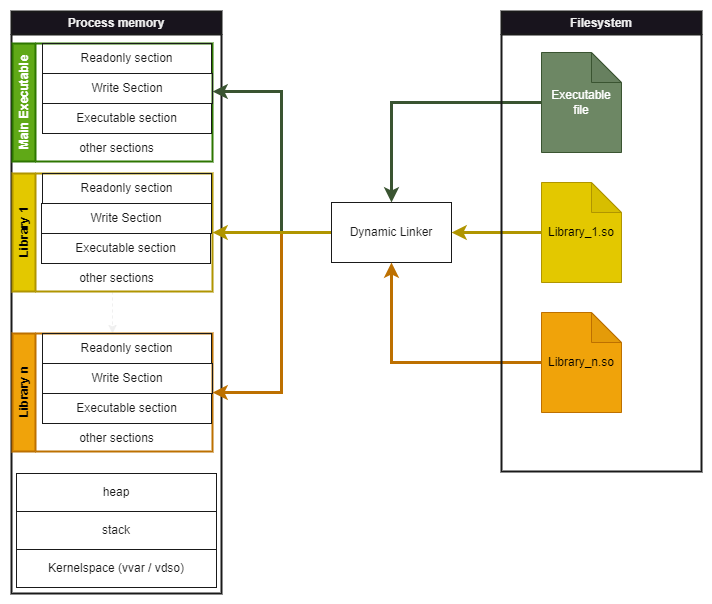
\includegraphics[width=1\linewidth]{linking.drawio.png}
        \caption{A simplified view of relation of process memory contents and their source}
        \label{fig:dyn-linking}
    \end{figure}

    \item {The /proc filesystem}

    The modern Linux system exposes a special \verb|/proc| directory.
    This is an interface that allows for file-based access to process memory and information.
    As an example, in a system that is currently running a process with a designated id of 2240 the system will provide a \verb|/proc/2240| directory, which will contain file interfaces for process memory, mappings, information, and other invaluable pieces of data.
    However, this directory is ephemeral, meaning that its contents can change and it will be destroyed upon the process' termination.
    Most important parts of every such folder are the \verb|maps| file which represent the segments, their mappings and their location in memory, and the \verb|mem| file which provides raw process memory access. \autoref{fig:proc-maps} illustrates how example process memory and its \verb|/proc| folder are related and how the information from the maps file represents placement, size, source and permissions of each segment loaded into a given process memory.
    
    \begin{figure}[h]
        \centering
        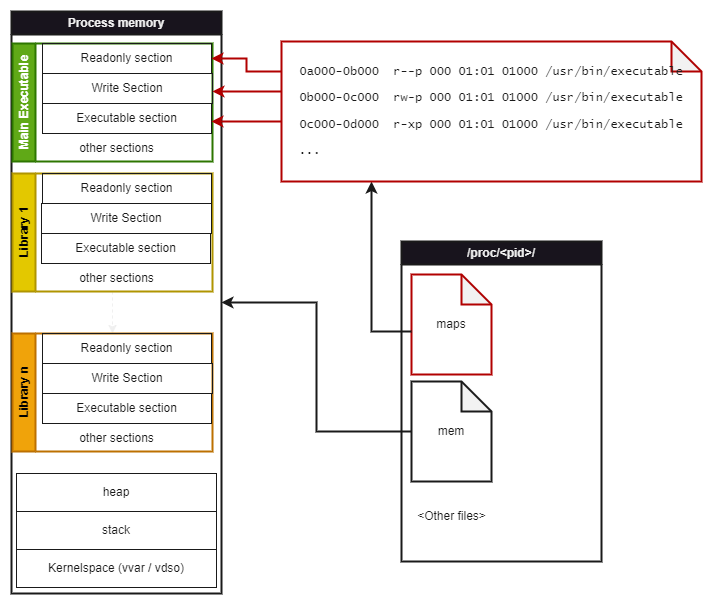
\includegraphics[width=1\linewidth]{proc-maps.drawio.png}
        \caption{Example relations of a running process to the /proc filesystem}
        \label{fig:proc-maps}
    \end{figure}

    \item {Rust language concepts}

    As the project is implemented in the Rust programming language, knowledge of some basic language concepts will enhance further readability for people unfamiliar with the language (more in the Rust book \cite{klabnik_rust_2023} or the language repository \cite{rust_foundation_rust-langrust_2024}):

    \subitem Struct - a data structure, it can have public and private fields, does not inherently contain any functions. However, traits and other functions can be implemented for it.

    \subitem Enum - a type composed of multiple types. Rust's extensive enum types can contain types within their variant or implement traits.

    \subitem Trait - similar to an interface defines a shared functionality, however, with some caveats. For the purpose of this text, treating it as such should suffice.

    \subitem Macros - Rust makes extensive use of macros for generating code (e.g. \verb|#[derive(debug)]| to automatically create a debug printable view of the struct) or providing extra functionality, for example, the \verb|matches!| macro to quickly verify whether the enum is of specific type.
\end{enumerate}